\documentclass[11pt]{article}

\usepackage[margin=1in]{geometry}
\usepackage{amsmath,amssymb}
\usepackage{booktabs}
\usepackage{graphicx}
\usepackage{hyperref}
\usepackage[capitalise,noabbrev]{cleveref}
\usepackage{xcolor}

\newcommand{\todo}[1]{\textcolor{red}{[TODO: #1]}}
\newcommand{\dRsq}{\Delta R^2}

% Numbers are generated from the run artifacts by paper/make_tables.py.
% macros.tex holds \newcommand definitions (preamble-safe); tables.tex holds
% the table environments and is included in the body. Never edit either by hand.
% AUTO-GENERATED by paper/make_tables.py -- do not edit by hand.
\newcommand{\NpairsTfive}{1,000,000}
\newcommand{\CeilingTfive}{0.9952}
\newcommand{\CeilingCross}{0.9634}
\newcommand{\RankMeEucl}{3.96}
\newcommand{\VarTopThree}{98.2}
\newcommand{\AucEucl}{0.9566}
\newcommand{\RecallDeploy}{0.189}
\newcommand{\RecallEndToEnd}{0.188}
\newcommand{\TieFraction}{54.0}
\newcommand{\DecisiveFraction}{46.0}
\newcommand{\ArbAcc}{0.7032}
\newcommand{\ArbGain}{+0.0576}
\newcommand{\DupSep}{0.1124}
\newcommand{\Nevents}{500}


\title{Diagnosing Learned Embeddings for Duplicate Track Removal\\
in Line Segment Tracking}
\author{Aiden Lee \\ \small (draft --- not for circulation)}
\date{\today}

\begin{document}
\maketitle

\begin{abstract}
Line Segment Tracking (LST) reconstructs charged-particle trajectories for the
CMS Phase-2 High Level Trigger, and removes duplicate track candidates using a
learned embedding trained with a contrastive loss. We do not propose a
replacement for that method; we diagnose it. Working from the same $500$-event
$t\bar{t}$ sample and the same feature definitions, we report four measurements
that the existing description does not contain. First, the embedding is
strongly rank-deficient: its effective rank is \RankMeEucl{} of $12$ dimensions,
with \VarTopThree\% of the variance in three principal components, which
accounts for the previously unexplained observation that increasing the
embedding dimension yields no improvement in test loss. Second, a globally
learned Mahalanobis precision matrix on top of such an embedding is a
reparameterisation of the Euclidean metric rather than a richer model, so the
common Euclidean-versus-Mahalanobis comparison is degenerate by construction; we
verify this numerically and give the conditions under which it fails. Third, the
$\dRsq<0.02$ window used to form candidate pairs is a blocking step with a
measurable recall ceiling of \CeilingTfive{} for T5--T5 pairs and \CeilingCross{}
for pLS--T5 pairs, which bounds every downstream recall figure. Fourth, balanced
pairwise AUC substantially overstates deployment performance: an AUC of
\AucEucl{} corresponds to an end-to-end duplicate recall of \RecallEndToEnd{} at
a realistic duplicate prior and a $99\%$ track-efficiency requirement. We
additionally show that duplicate decisions taken pairwise are globally
inconsistent, and that the choice of which duplicate to discard --- currently a
fixed collection priority --- is learnable.
\end{abstract}

\section{Introduction}
\label{sec:intro}

Line Segment Tracking~\cite{lst2022,segmentlinking} builds track candidates
hierarchically from mini-doublets and triplets into quintuplets (T5), and
combines these with pixel line segments (pLS) from an upstream pixel iteration.
Because the same simulated particle can be reconstructed by several candidates,
and because candidates from different collections may describe the same
trajectory, the final candidate list must be cleaned of duplicates. In
production this is done by ``cross-cleaning'': candidates close in $\eta$--$\phi$
are compared, and a fixed collection priority (pT5 $>$ pT3 $>$ T5 $>$ pLS)
decides which survives.

A learned component was added to this step~\cite{dp2025048}: two networks embed
T5 ($30$ features) and pLS ($10$ features) candidates into a shared $6$-dimensional
space, and the Euclidean distance between embeddings enters a contrastive
loss~\cite{hadsell2006} that pulls duplicates together and pushes non-duplicates
apart. The method is deployed, and reduces the duplicate rate by up to $50\%$
for displaced tracks at a throughput cost of $3$--$4\%$.

This paper is diagnostic. We take that method as given and ask what its
behaviour actually is, using measurements that are standard elsewhere in machine
learning but have not been applied here. Our contributions are:

\begin{enumerate}
\item \textbf{The embedding is rank-deficient} (\cref{sec:collapse}). Its
  effective rank~\cite{rankme} is roughly half its nominal dimension. This
  explains, mechanistically, why raising the embedding dimension does not help
  --- an observation reported in~\cite{dp2025048} without explanation.
\item \textbf{The Euclidean-versus-Mahalanobis comparison is degenerate}
  (\cref{sec:gauge}). We show, and verify numerically, that a globally learned
  precision matrix on top of an encoder ending in a trainable linear layer adds
  no expressive power. We give the three conditions under which this ceases to
  hold, and a per-instance alternative that escapes it.
\item \textbf{The pairing window has a measurable recall ceiling}
  (\cref{sec:ceiling}), and \textbf{balanced AUC overstates deployment
  performance} (\cref{sec:operating}).
\item \textbf{Pairwise decisions are globally inconsistent}
  (\cref{sec:transitivity}), and \textbf{arbitration is learnable}
  (\cref{sec:arbitration}). We also calibrate the decision threshold with a
  distribution-free guarantee on efficiency loss (\cref{sec:conformal}).
\end{enumerate}

\paragraph{Relation to prior work.}
We claim neither the learned-embedding approach~\cite{dp2025048} nor learned
duplicate arbitration in tracking, which has been demonstrated in ACTS using a
clustering step followed by a ranking network~\cite{allaire2025,allaire2023}.
The equivalence in \cref{sec:gauge} is a known result for linear metric
learning~\cite{lmnn,kulis2013,bellet2013}; our contribution is to observe that it
survives a deep encoder and therefore applies to the deployed configuration, and
to quantify its consequences. Related recent work introduces pair-conditioned
Mahalanobis metrics in a different domain~\cite{pamd}, and the ``gauge freedom''
framing for neural representations~\cite{cain2026}.

\section{Setup}
\label{sec:setup}

\paragraph{Data.} A sample of \Nevents{} simulated $t\bar{t}$ events at
HL-LHC pileup. T5 candidates are described by the $30$ features of
\cite{dp2025048}: per-anchor-hit $\eta$, $\phi$, $z$, $r$ differences along the
candidate, inverse inner/bridge/outer radii, and the T3 fake/prompt/displaced
scores with their differences. pLS candidates use $10$ features including
$\eta$, its fitted error, $\phi$, inverse $p_T$, and circle-fit quantities.

\paragraph{Pairs.} Candidate pairs are formed within $\dRsq<0.02$, matching the
production cross-cleaning window. A pair is labelled \emph{duplicate} if both
members match the same simulated track index. We generate \NpairsTfive{} T5--T5
pairs. Pair sampling is capped per event, which we show
in \cref{sec:transitivity} has consequences for graph-level measurements.

\paragraph{Training.} Each metric is trained with its \emph{own} pair of encoders
under its \emph{own} objective. This matters: sharing one encoder across metrics,
or reading a differently-trained embedding out with a new distance, produces
numbers that reflect the training objective rather than the metric. Encoders are
$30{\to}128{\to}64{\to}d$ with batch normalisation and no terminal nonlinearity.
The margin is set from the scale the embedding actually occupies rather than
fixed a priori. This is a live failure mode in both directions: a margin far
above the embedding scale leaves the repulsive term permanently unsaturated,
while a margin far below it clamps that term to zero and removes the repulsive
gradient entirely, after which the embedding collapses. We therefore log the
fraction of non-duplicate pairs still inside the margin each epoch and treat
values near $0$ or $1$ as a failed run; all results reported here held this
fraction between $0.29$ and $0.56$.

\section{The embedding is rank-deficient}
\label{sec:collapse}

We measure the effective rank of the embedding using
RankMe~\cite{rankme}, the exponentiated Shannon entropy of the normalised
singular-value spectrum,
\begin{equation}
\mathrm{RankMe}(Z) = \exp\!\left(-\sum_k p_k \log p_k\right),
\qquad p_k = \frac{\sigma_k(Z)}{\lVert \sigma(Z)\rVert_1} + \epsilon ,
\end{equation}
which equals the nominal dimension for an isotropic embedding and $1$ for a fully
collapsed one. \Cref{tab:metrics} reports it for each metric.

The Euclidean embedding attains an effective rank of \RankMeEucl{} out of $12$,
with \VarTopThree\% of the variance in three components. This is dimensional
collapse in the sense of~\cite{jing2022}: under a contrastive objective the
gradient on each singular direction is proportional to that direction's own
singular value, so directions that begin small remain small.

\paragraph{Consequence: the dimension scan measures collapse, not sufficiency.}
Ref.~\cite{dp2025048} reports that ``increasing the embedding dimension up to
$32$ shows no improvement in test loss for either model'', based on a scan over
embedding sizes with five random seeds. That is usually read as evidence that six
dimensions suffice. We tested the alternative reading directly by sweeping
$d \in \{4,6,8,12,16,32\}$ (\cref{fig:dimsweep}, \cref{tab:dimsweep}).

The Euclidean embedding's effective rank is essentially independent of $d$:
over an eight-fold increase in nominal dimension it rises only from $3.47$ to
$4.44$, a factor of $1.28$, while balanced AUC is flat to the fourth decimal
($0.9551$ at $d=4$, $0.9554$ at $d=32$). We therefore reproduce the reported null
result and supply its mechanism: the additional dimensions are never populated,
so they cannot contribute. At the deployed $d=6$ the embedding uses an effective
$3.59$ of its six dimensions.

The same sweep shows this is a property of the metric and not of the task. Under
a cosine objective the effective rank tracks the nominal dimension over the same
range, rising from $3.93$ to $20.78$ --- a factor of $5.28$ against the $1.28$ of
the Euclidean case --- at equal or better discrimination. Six dimensions are not
``enough''; six dimensions are what the Euclidean objective can fill.

\paragraph{Replication.} Trained independently on two disjoint halves of the
events, the effective rank agrees to $4.87$ versus $4.82$ (Euclidean) and $10.26$
versus $10.49$ (cosine), with balanced AUC agreeing to $0.003$. The separation
between the two metrics is an order of magnitude larger than the spread between
halves. This controls for subset and seed instability only; it shares whatever
biases the sample carries and is not a test of external validity.

\begin{figure}[t]
\centering
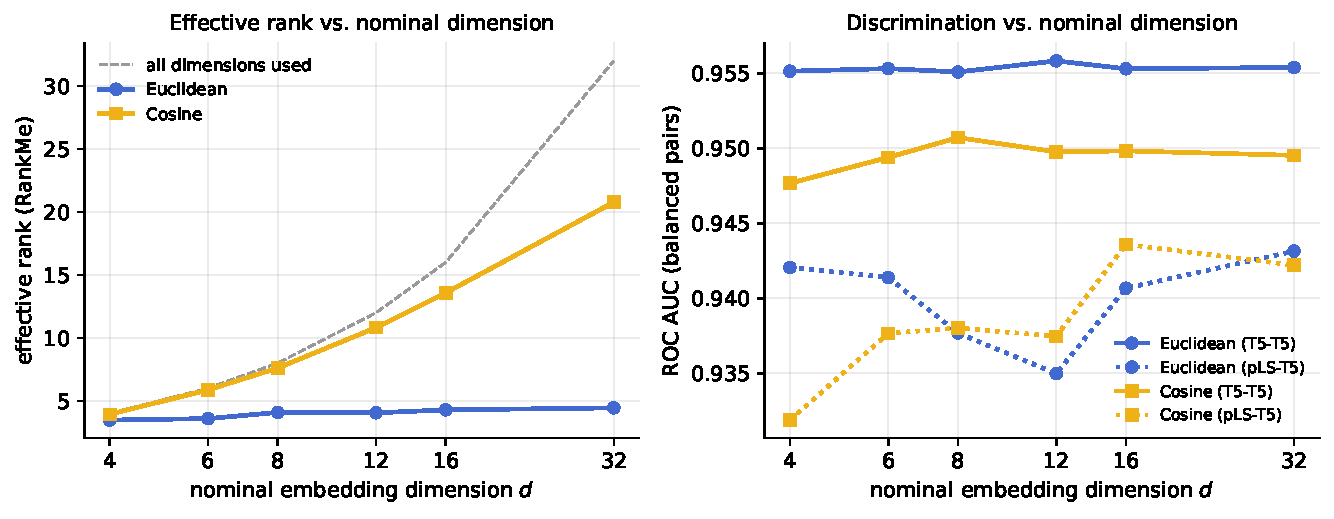
\includegraphics[width=\textwidth]{fig_dimsweep}
\caption{Effective rank and discrimination against nominal embedding dimension.
The dashed diagonal is the locus an embedding using all of its dimensions would
follow. The Euclidean embedding departs from it immediately and is flat beyond
$d\approx8$, while the cosine embedding continues to track it. Balanced AUC
(right) is insensitive to $d$ for both metrics, which is the reported null result
that the left panel explains.}
\label{fig:dimsweep}
\end{figure}

\paragraph{The metric choice determines whether collapse happens.}
\Cref{tab:metrics} shows the effect is not uniform across metrics. The cosine
embedding retains an effective rank of $11.05$ of $12$ where the Euclidean one
retains \RankMeEucl{}, and it does so at no cost in discrimination: cosine matches
Euclidean on T5--T5 pairs and is substantially better on the cross-collection
pLS--T5 pairs ($0.9493$ versus $0.9004$). Cosine is scale-invariant, so the
direction along which the Euclidean embedding expands --- and which comes to
dominate its spectrum --- simply does not exist for it. On this evidence, a
cosine objective is the better default for this task.

\paragraph{A variance floor does not prevent rank collapse.}
It is tempting to prevent collapse with VICReg's variance term~\cite{vicreg},
which lower-bounds each dimension's standard deviation. We find this insufficient:
with every per-dimension variance held inside its bounds, the effective rank still
falls to \RankMeEucl{} and the leading three components still carry
\VarTopThree\% of the variance. Rank collapse here is driven by \emph{correlation
between} dimensions, not by any dimension's marginal variance vanishing, and only
a covariance penalty addresses that. This creates a genuine tension with
\cref{sec:gauge}: a covariance penalty drives $\mathrm{cov} \to I$ and hence
$V \to I$, so the very regulariser that would prevent collapse also trivialises
the learned precision matrix. One cannot have both.

\paragraph{Scale.} A second, related defect: the embedding occupies a scale far
below the contrastive margin, so essentially every pair sits inside the margin
and the repulsive term never saturates. Setting the margin from the data scale,
or removing it entirely in favour of a learned decision scale~\cite{hib},
eliminates this class of error by construction.

\section{A global learned metric is a reparameterisation}
\label{sec:gauge}

Write a positive-definite precision matrix as $V = L^\top L$. If the encoder ends
in a trainable linear layer with weight $W$ and bias $c$, then for any pair the
bias cancels in the difference and
\begin{equation}
d_V\big(f(a), f(b)\big)^2
 = \big(W(h_a - h_b)\big)^\top V \big(W(h_a-h_b)\big)
 = \big\lVert LW (h_a - h_b) \big\rVert^2 .
\label{eq:gauge}
\end{equation}
Since $LW$ is itself an admissible weight matrix, the model class
$\{\text{encoder ending in } W,\ \text{metric } V\}$ equals
$\{\text{encoder ending in } LW,\ \text{metric } I\}$. A globally learned
precision matrix therefore adds no expressive power over the Euclidean metric; it
is unidentifiable in every direction except overall scale.

We verify \cref{eq:gauge} numerically. Planting the exact solution $LW$ reproduces
the Mahalanobis distances to a relative error of $1.6\times10^{-13}$; fitting the
same family from scratch reaches a normalised residual of $0.00000$, whereas the
same family cannot reproduce a per-instance metric (residual $0.358$, converged).

\paragraph{When this fails.} The equivalence is not universal, and the boundaries
matter for anyone applying it:
\begin{itemize}
\item A \emph{terminal nonlinearity} breaks it (relative error $0.42$), because
  the metric can no longer be commuted through the final map.
\item \emph{$L_2$ normalisation} breaks it (relative error $0.955$), since
  $Lx/\lVert Lx\rVert \neq L(x/\lVert x\rVert)$. Metric-learning pipelines that
  normalise onto the unit hypersphere are therefore unaffected.
\item \emph{Weight decay} preserves the distances but not the optimisation
  problem: $\lVert W\rVert_F^2$ and $\lVert LW\rVert_F^2$ differ by a factor of
  $13.3$ in our test. The function classes coincide; the regularised problems do
  not.
\end{itemize}
The deployed configuration~\cite{dp2025048} has an unnormalised, linear-output
embedding, so the equivalence applies to it.

\paragraph{What does add capacity.} The absorption argument fails as soon as the
precision depends on the input, because no fixed weight can absorb a
pair-dependent transform. The cheapest such model predicts a diagonal
log-variance per candidate and scores pairs by the mutual likelihood
score~\cite{pfe},
\begin{equation}
s(i,j) = -\tfrac{1}{2}\sum_l \left[
\frac{(\mu_i^l - \mu_j^l)^2}{\sigma_i^2(l)+\sigma_j^2(l)}
+ \log\big(\sigma_i^2(l)+\sigma_j^2(l)\big)\right],
\end{equation}
whose effective precision $1/(\sigma_i^2+\sigma_j^2)$ is per-pair and whose
log-determinant term has no representation as a distance on the means. This costs
one additional linear head.

\section{The pairing window has a recall ceiling}
\label{sec:ceiling}

The $\dRsq<0.02$ window is a \emph{blocking} step in the entity-resolution
sense~\cite{deepblocker}: any true duplicate pair whose members fall outside it is
never presented to the model and cannot be recovered, whatever the model does.
Blocking recall is routinely reported in that literature and bounds every
downstream figure, but is not reported for tracking.

Enumerating all true duplicate pairs and asking what fraction falls inside the
window, we measure a ceiling of \CeilingTfive{} for T5--T5 pairs and
\CeilingCross{} for pLS--T5 pairs. The cross-collection ceiling is the tighter of
the two, which is consistent with pLS and T5 candidates for the same particle
being separated further in $\eta$--$\phi$ than two T5 candidates are.

\section{Balanced AUC overstates deployment performance}
\label{sec:operating}

Pair sampling is balanced $50/50$ by construction, whereas the deployed duplicate
prior among in-window pairs is a few percent. Because AUC is prior-invariant and
integrates over operating points that would never be deployed, it is close to
uninformative about deployment.

\Cref{tab:operating} re-evaluates each metric at a realistic prior, at the
operating point that preserves $99\%$ of genuine tracks --- the quantity that
matters, since discarding a non-duplicate destroys a real particle track. A
balanced AUC of \AucEucl{} corresponds to an in-window duplicate recall of
\RecallDeploy{}, and \RecallEndToEnd{} once the blocking ceiling is folded in.

\section{Pairwise decisions are globally inconsistent}
\label{sec:transitivity}

``Is the same particle as'' is an equivalence relation and must be transitive, but
a pairwise scorer has no mechanism enforcing this~\cite{binette2020}. We count
\emph{closed} triples --- those for which all three pairs were actually scored ---
and ask how many violate transitivity by asserting $a\sim b$ and $b\sim c$ while
denying $a\sim c$. Triples with an unscored edge are excluded rather than counted
as denials.

Ground-truth labels give $108{,}465{,}681$ closed triples over $40$ densely-paired
events and exactly zero violations, confirming the measurement. The trained model
is intransitive on $4.0\%$ to $17.5\%$ of closed triples depending on the
operating threshold.

\paragraph{A sampling caveat.} With the per-event pair cap used in the standard
configuration, $98.6\%$ of triples have an unscored edge and the measurement is
starved. Generating all in-window pairs instead reduces this to $0.40\%$, and the
figures above use that dense configuration. Anyone repeating this measurement
must do the same, or the result will be an artefact of the sampling rather than a
property of the scorer.

\section{Arbitration is learnable}
\label{sec:arbitration}

The embedding answers a symmetric question --- are these the same particle? ---
whereas duplicate removal requires an asymmetric one: which candidate survives?
Production answers the second with a fixed collection priority, which carries no
information at all for same-collection pairs.

We score a pair with
$s(i,j) = g(e_i,e_j) - g(e_j,e_i)$, which is antisymmetric by construction for
any weights, so the decision cannot depend on the arbitrary order in which pairs
were enumerated. The target is $t5\_pMatched$, the fraction of a candidate's hits
belonging to its matched simulated track.

This quantity is quantised to ten values and \TieFraction\% of duplicate pairs
are exact ties, which carry no arbitration signal and are excluded from training;
the remaining \DecisiveFraction\% are usable. \Cref{tab:arbiter} reports
accuracy by input representation. The head reaches \ArbAcc{} against $0.5$ for
the priority rule.

\paragraph{The embedding discards what the arbiter needs.} Raw features add
\ArbGain{} accuracy over the embedding alone. This is expected rather than
surprising: the contrastive objective explicitly minimises $\lVert e_i - e_j\rVert$
over duplicates, so in the limit where it succeeds the antisymmetric score is
identically zero. We measure duplicate pairs separated to \DupSep{} of the
embedding scale. The better the embedding is at its own task, the less
arbitration information it retains --- so an arbiter must read raw features.

\section{A threshold with a distribution-free guarantee}
\label{sec:conformal}

Production uses hand-tuned $\eta$-binned working points with no statistical
guarantee. Since discarding a non-duplicate destroys a real track, the operating
question is precisely one of risk control: what threshold removes at most a
stated fraction of genuine tracks?

Conformal risk control~\cite{crc} answers this. For per-event losses
$L_i(\lambda)$ that are non-increasing in $\lambda$ and bounded by $B$,
\begin{equation}
\hat{\lambda} = \inf\Big\{\lambda : \tfrac{n}{n+1}\hat{R}_n(\lambda) + \tfrac{B}{n+1} \le \alpha \Big\}
\end{equation}
guarantees $\mathbb{E}[L(\hat\lambda)] \le \alpha$ under exchangeability alone.

Two points deserve emphasis. The exchangeable unit is the \emph{event}, not the
pair: pairs within an event share a collision and are strongly dependent, and
calibrating on pairs inflates the effective sample size by the pairs-per-event
factor. In simulation, event-level calibration controls the risk (mean $0.0059$
against $\alpha=0.01$) while pooled-pair calibration violates it ($0.0103$).

Second, the finite-sample penalty $B/(n+1)$ is paid before any data is seen. With
$500$ events, half held out for calibration, and the naive bound $B=1$, it is
$1/251 = 0.004$, so $\alpha=0.005$ has $80\%$ of its budget consumed up front and
$\alpha \le 0.002$ is uncertifiable. Restricting the threshold grid to a range
that would plausibly be deployed tightens $B$ and, counter-intuitively, certifies
a \emph{more} aggressive threshold, because budget is freed from a worst case that
would never occur.

% AUTO-GENERATED by paper/make_tables.py -- do not edit by hand.

\begin{table}[t]
\centering
\caption{Metric comparison with each metric trained independently under its own
objective. RankMe is the effective rank of the 12-dimensional embedding
(\cref{sec:collapse}); var@3 is the variance captured by the leading three
principal components.}
\label{tab:metrics}
\begin{tabular}{lcccc}
\toprule
Metric & AUC (T5--T5) & AUC (pLS--T5) & RankMe & var@3 \\
\midrule
Euclidean & 0.9566 & 0.9004 & 3.96 & 98.2\% \\
Mahalanobis & 0.9297 & 0.7046 & 7.47 & 87.3\% \\
Cosine & 0.9566 & 0.9493 & 11.05 & 56.1\% \\
\bottomrule
\end{tabular}
\end{table}

\begin{table}[t]
\centering
\caption{Balanced-pair AUC against deployment-relevant performance at a
5\% duplicate prior and $99\%$ track efficiency. End-to-end
recall folds in the blocking ceiling of the $\Delta R^2<0.02$ window.}
\label{tab:operating}
\begin{tabular}{lcccc}
\toprule
Metric & Balanced AUC & Recall (in-window) & Ceiling & Recall (end-to-end) \\
\midrule
Euclidean & 0.9566 & 0.189 & 0.9952 & 0.188 \\
Mahalanobis & 0.9297 & 0.185 & 0.9952 & 0.184 \\
Cosine & 0.9566 & 0.189 & 0.9952 & 0.188 \\
\bottomrule
\end{tabular}
\end{table}

\begin{table}[t]
\centering
\caption{Arbitration accuracy by input representation. The collection-priority
rule carries no information for same-collection pairs and is a coin flip by
construction. The trained embedding separates duplicate pairs to
$0.1124$ of the embedding scale, which is why the embedding-only head
underperforms.}
\label{tab:arbiter}
\begin{tabular}{lccc}
\toprule
Input & Accuracy & Accuracy (decisive half) & Ranking AUC \\
\midrule
Embedding only & 0.6456 & 0.7619 & 0.7291 \\
Raw features & 0.7032 & 0.8549 & 0.8071 \\
Embedding + raw & 0.7032 & 0.8498 & 0.8073 \\
Collection priority (baseline) & 0.5000 & 0.5000 & 0.5000 \\
\bottomrule
\end{tabular}
\end{table}

\begin{table}[t]
\centering
\caption{Effective rank and discrimination against nominal embedding dimension.
Effective rank saturates while the nominal dimension grows by a factor of eight,
which is what makes additional dimensions inert.}
\label{tab:dimsweep}
\begin{tabular}{cccccccc}
\toprule
& \multicolumn{3}{c}{Euclidean} & \multicolumn{3}{c}{Cosine} \\
\cmidrule(lr){2-4}\cmidrule(lr){5-7}
$d$ & RankMe & AUC (T5) & AUC (pLS) & RankMe & AUC (T5) & AUC (pLS) \\
\midrule
4 & 3.47 & 0.9551 & 0.9421 & 3.93 & 0.9477 & 0.9319 \\
6 & 3.59 & 0.9553 & 0.9414 & 5.87 & 0.9494 & 0.9377 \\
8 & 4.08 & 0.9551 & 0.9377 & 7.61 & 0.9507 & 0.9380 \\
12 & 4.05 & 0.9558 & 0.9350 & 10.81 & 0.9498 & 0.9375 \\
16 & 4.28 & 0.9553 & 0.9407 & 13.58 & 0.9498 & 0.9436 \\
32 & 4.44 & 0.9554 & 0.9431 & 20.78 & 0.9495 & 0.9422 \\
\bottomrule
\end{tabular}
\end{table}


\section{Limitations}
\label{sec:limitations}

The equivalence of \cref{sec:gauge} is a known result for linear metric
learning~\cite{lmnn,kulis2013}; we extend its scope and quantify consequences
rather than establishing it. The intransitivity and blocking-ceiling
measurements are properties of this pipeline and sample and need not transfer.
All results use a single $t\bar{t}$ sample at one pileup. We replicate the
central measurements on two disjoint halves of the events, which controls for
subset and seed instability but cannot detect a bias shared by the whole sample;
external validity across pileup and physics process remains untested. The
conformal guarantee requires exchangeability and does not survive a pileup shift,
which we demonstrate. We do not report end-to-end tracking efficiency, fake rate, or
throughput against the production baseline; those require integration into the
CMSSW sequence and are the natural next step. \todo{integrate and report MTV
efficiency/fake/duplicate versus $p_T$, $\eta$, $|d_{xy}|$ at matched efficiency}

\section{Conclusion}

The deployed learned embedding for LST duplicate removal works, and we do not
propose replacing it. We do show that it is operating in a rank-collapsed regime
that explains its own reported insensitivity to embedding dimension; that the
natural next step of learning a global metric on top of it cannot help, for
reasons that are structural rather than empirical; that its pairing window
imposes a quantifiable recall ceiling; that its headline evaluation metric
substantially overstates deployment performance; and that the one decision it
leaves to a fixed heuristic --- which duplicate to keep --- is learnable from
data already present in the sample.

\begin{thebibliography}{99}

\bibitem{lst2022} P.~Chang \emph{et al.},
  ``Line Segment Tracking in the HL-LHC,'' arXiv:2207.08207.

\bibitem{segmentlinking} P.~Chang \emph{et al.},
  ``Segment Linking: A Highly Parallelizable Track Reconstruction Algorithm for
  HL-LHC,'' J.\ Phys.\ Conf.\ Ser.\ \textbf{2375}, 012005 (2022),
  arXiv:2209.13711.

\bibitem{dp2025048} CMS Collaboration,
  ``Extended ML Selections and Track Embeddings for Duplicate Removal in Line
  Segment Tracking (LST),'' CMS-DP-2025-048, CERN, 2025.

\bibitem{hadsell2006} R.~Hadsell, S.~Chopra, Y.~LeCun,
  ``Dimensionality Reduction by Learning an Invariant Mapping,'' CVPR 2006.

\bibitem{vicreg} A.~Bardes, J.~Ponce, Y.~LeCun,
  ``VICReg: Variance-Invariance-Covariance Regularization for Self-Supervised
  Learning,'' arXiv:2105.04906.

\bibitem{rankme} Q.~Garrido \emph{et al.},
  ``RankMe: Assessing the Downstream Performance of Pretrained Self-Supervised
  Representations by their Rank,'' arXiv:2210.02885.

\bibitem{jing2022} L.~Jing \emph{et al.},
  ``Understanding Dimensional Collapse in Contrastive Self-supervised
  Learning,'' arXiv:2110.09348.

\bibitem{lmnn} K.~Q.~Weinberger, L.~K.~Saul,
  ``Distance Metric Learning for Large Margin Nearest Neighbor
  Classification,'' JMLR \textbf{10}, 207--244 (2009).

\bibitem{kulis2013} B.~Kulis,
  ``Metric Learning: A Survey,'' Found.\ Trends Mach.\ Learn.\ \textbf{5}(4),
  287--364 (2013).

\bibitem{bellet2013} A.~Bellet, A.~Habrard, M.~Sebban,
  ``A Survey on Metric Learning for Feature Vectors and Structured Data,''
  arXiv:1306.6709.

\bibitem{pamd} D.~Roh, J.~Bae, H.-L.~Choi,
  ``PAMD: Structured Adaptive Distances for Bisimulation Representations in
  Visual Reinforcement Learning,'' arXiv:2607.18004.

\bibitem{cain2026} J.~Cain,
  ``Gauge Freedom and Metric Dependence in Neural Representation Spaces,''
  arXiv:2603.06774.

\bibitem{pfe} Y.~Shi, A.~K.~Jain,
  ``Probabilistic Face Embeddings,'' arXiv:1904.09658.

\bibitem{hib} S.~J.~Oh \emph{et al.},
  ``Modeling Uncertainty with Hedged Instance Embedding,'' arXiv:1810.00319.

\bibitem{allaire2023} C.~Allaire, F.~Bouvet, H.~Grasland, D.~Rousseau,
  ``Ranking-based neural network for ambiguity resolution in ACTS,''
  EPJ Web Conf.\ \textbf{295}, 03022 (2024), arXiv:2312.05070.

\bibitem{allaire2025} C.~Allaire, F.~Bouvet, H.~Grasland, D.~Rousseau,
  ``Ranking-based machine learning for track seed selection in ACTS,''
  EPJ Web Conf.\ \textbf{337}, 01025 (2025).

\bibitem{deepblocker} S.~Thirumuruganathan \emph{et al.},
  ``Deep Learning for Blocking in Entity Matching: A Design Space Exploration,''
  PVLDB \textbf{14}(11), 2459--2472 (2021).

\bibitem{binette2020} O.~Binette, R.~C.~Steorts,
  ``(Almost) All of Entity Resolution,'' arXiv:2008.04443.

\bibitem{crc} A.~N.~Angelopoulos, S.~Bates, A.~Fisch, L.~Lei, T.~Schuster,
  ``Conformal Risk Control,'' arXiv:2208.02814.

\end{thebibliography}

\end{document}
